%!TEX root = main.tex
\section{Materials and Methods}

\subsection{Datasets: ELSDSR and TIMIT}

Two datasets were used for speaker classification; ELSDSR and TIMIT. The ELSDSR dataset includes 23 people and was specifically created for automatic speaker recognition. The TIMIT dataset is an acoustic-phonetic speech corpus and was thus not directly created for automatic speaker recognition. As a result, the TIMIT dataset has people with few observations or very short soundclips. To alleviate potential problems this might cause for speaker classification the dataset was filtered to only include people with sufficiently many long observations. After this filtering 81 people were left.

Both datasets were preprocessed by normalizing the energy (L2 norm) of each spectrogram to be one and then globally normalizing the data to have $\mu = 0$ and $\sigma = 1$.

\subsection{The Dieleman network}

The Dieleman network, expecting a spectrogram $x \in \mathbb{R}^{m \times n}$ as input, consists of 6 layers: 2 $\times$(\emph{Convolutional} layer + \emph{Max Pooling} layer), followed by 2 consecutive fully connected \emph{Dense} layers.

The 1st Convolutional layer contains $32$ filters (kernels) of dimension $m \times 8$. Each filter only convolutes along the time axis with a stride of $1$ computing a single value for each stride offset, resulting in an output of size $n - \frac{8}{2} + 1 = n - 3$ for each filter (i.e. the output of layer 1 is of dimension $32 \times (n-3)$). This is illustrated in \cref{fig:convolution-1}.

\begin{figure}[H]
  \centering
  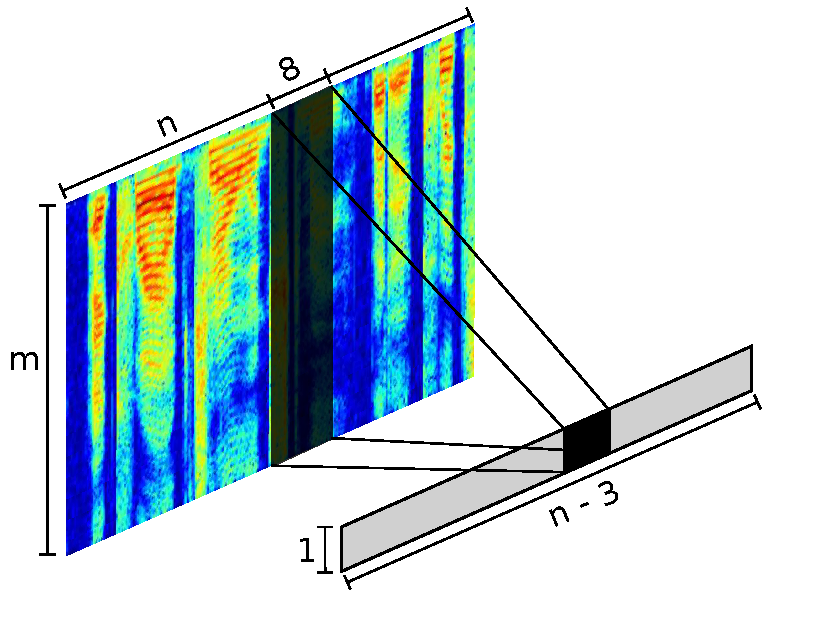
\includegraphics[width=0.4\textwidth]{inkscape/convolution.pdf}
  \caption{Illustration of 1st convolution layer for a single filter.}
  \label{fig:convolution-1}
\end{figure}

The 2nd layer performs a 1-dimensional max pooling of size $1 \times 4$ on the output from layer 1. Thus, for each filter in layer 1 a window of size $1 \times 4$ is slid through the filter output with a stride offset of $4$ extracting the maximum value in the window.

This reduces the dimensionality of the output by $4$ giving a layer output of size $32 \times \frac{1}{4}(n-3)$.

For the 3rd and 4th network layer the same procedure is applied using filters of size $1 \times 8$ and again a max pooling of size $1 \times 4$.

Finally the output of layer 4 is fed into a regular fully-connected dense layer of $100$ nodes followed by a final softmax function layer.

In the \emph{Convolutional} and \emph{Dense} layers the rectifier function (\cref{eq:rectifier}) is used as activation function (sometimes also refered to as Rectified Linear Unit (ReLU)).
\begin{equation}
  f(x) = \text{max(}0, x\text{)},
  \label{eq:rectifier}
\end{equation}


The network is implemented in \texttt{python} using the library \texttt{lasagne}, which is implemented on top of \texttt{Theano} which allows for the use of highly optimized mathematical expression implementations and for transparent use of GPUs \cite{theano}.

\subsection{Scale Invariant Regularization}

In order to train the network a loss function measuring the performance has to be chosen. Since needs to classify $k$-classes the cross-entropy loss is chosen:
\begin{equation}
\mathcal{L}_{entropy} = - \frac{1}{N} \sum_{i=1}^N \sum_{k=1}^K t_{i,k} \ln(P(C_{i,k} | x_i, w))
\end{equation}

In addition, \cite{scale-invariante} proposes that a the learned model should be invariant to small transformations of the input data. This can be accomplished by adding a transformation invariant regularizers to the loss function. Let $s(x, \alpha)$  be a tranformation where $x$ is the observation and $\alpha$ is a parameterization of the transformation. Furthermore let $s$ be defined such that $s(x, 0) = x$. As such two examples of $s$ are:
\begin{align}
\text{scale transformation:}&\quad s(x, \alpha) = (1+\alpha) x\\
\text{offset transformation:}&\quad s(x, \alpha) = x + \alpha
\end{align}

The regularizer can then be constructed by penalizing changes in the output function (in this case $P(C_{i, k})$) by minimizing the derivative of the output function with respect to $\alpha$.
\begin{equation}
\mathcal{R}(s) = \frac{1}{N} \sum_{i=1}^N \left. \frac{\partial P(C_{i, k} | s(x_i, \alpha), w)}{\partial \alpha} \right|^2_{\alpha=0}
\end{equation}
By using the chain rule the derivative can be expressed as:
\begin{equation*}
\left. \frac{\partial P(C_{i, k} | s(x_i, \alpha), w)}{\partial \alpha} \right|_{\alpha=0} = \left.\nabla_x P(C_{i, k} |  x_i, w) \frac{\partial s(x_i, \alpha)}{\partial \alpha} \right|_{\alpha=0}
\end{equation*}

This is extremely convenient from an implementation perspective,as $P(C_{i, k} | x_i, w)$ is already expressed in the Theano graph. More concretely for the scale and offset invariance the regularizers become:
\begin{align}
\text{scale invariant: }& \mathcal{R} = \frac{1}{N} \sum_{i=1}^N \left(\nabla_x P(C_{i, k} | x_i, w) \bigcdot x_i\right)^2 \\
\text{offset invariant: }& \mathcal{R} = \frac{1}{N} \sum_{i=1}^N \left(\nabla_x P(C_{i, k} | x_i, w) \bigcdot \mathbf{1}\right)^2
\end{align}

The full loss function is then $\mathcal{L} = \mathcal{L}_{entropy} + \lambda \mathcal{R}$ where $\lambda$ is a regularization parameter.
